\documentclass[11pt, a4paper, norsk]{rapport1} % change ``USenglish'' to ``norsk'' if applicable.

\setlength{\marginparwidth}{2cm} % Set marginparwidth to avoid issues with todonotes.
\usepackage{kyblab} % Contains all included packages. See kyblab.sty.
\addbibresource{bibliography.bib} % Makes the bibliography file available to biblatex.
\begin{document}

% Example citation
\nocite{*}

% Titlepage
\title{TTK4111 - Oblig 5}
\author{Fredrik Warø}
\date{Date: 22/10/2024}
\begin{titlepage}
    \maketitle
    \begin{figure}
    \centering
    \end{figure}
    \thispagestyle{empty}
\end{titlepage}
    Alt av simuleringer og kode finnes i \url{https://github.com/fredrswa/TTK4111-Oblig-5}
%\newpage

% Bibliography


% Abstract
%\newpage
%\thispagestyle{empty} % Avoid page numbering on the abstract page.

% TOC
%\newpage
%\tableofcontents
%\thispagestyle{empty} % Avoid page numbering on the table of contents.

% Main content

%\newpage
\setcounter{page}{1} % Set the page counter to 1.

\section{Oppgaver}
\subsection{Oppgave 1}
Systemet er gitt i ligningsettet \ref{eq:1}.
\begin{equation}
    \label{eq:1}
    \begin{aligned}
        M\ddot{p} &= sin(\theta)(F_1 + F_2) \\
        M\ddot{h} &= cos(\theta)(F_1 + F_2) - Mg \\
        J\ddot{\theta} &= l(F_2 - F_1) \\
    \end{aligned}
\end{equation}
Pådraget er gitt ved ligning \ref{eq:2}.
\begin{equation}
    \label{eq:2}
    u_h = F_1 + F_2 - Mg, \quad u_\theta = F_1 - F_2 \\
\end{equation}
\textbf{(a)}
Hviklet gir følgende ligninger for kreftene \ref{eq:3}.
\begin{equation}
    \begin{aligned}
        \label{eq:3}
        F_1 &= \frac{1}{2}u_h + \frac{1}{2}u_\theta + \frac{Mg}{2} \\
        F_2 &= \frac{1}{2}u_h - \frac{1}{2}u_\theta + \frac{Mg}{2} \\
    \end{aligned}
\end{equation}
\textbf{(b)} Gitt at $|\theta| \ll 1$ og $ u_h\ll 1$ kan vi anta at $sin(\theta) \approx \theta$ og $cos(\theta) \approx 1$. Dette gir oss ligningsettet \ref{eq:4}.
\begin{equation}
    \label{eq:4}
    \begin{aligned}
        M\ddot{p} &= \theta(F_1 + F_2) \\
        M\ddot{h} &= (F_1 + F_2) - Mg \\
        J\ddot{\theta} &= l(F_2 - F_1) \\
    \end{aligned}
\end{equation}
Ligning \ref{eq:3} og \ref{eq:4} gir oss ligningsettet \ref{eq:5}.
\begin{equation}
    \begin{aligned}
        \label{eq:5}
        \ddot{p} &= M^{-1}\theta(u_h + Mg)  = \theta g\\
        \ddot{h} &= M^{-1}(u_h + Mg) - g  = M^{-1}u_h\\
        J\ddot{\theta} &= 2l(u_\theta) \\
    \end{aligned}
\end{equation}
\textbf{(c)} Vi starter med å løse overføringsfunksjonen fra $u_\theta$ til $\theta$.
\begin{equation}
    \label{eq:6}
    s^2\hat{\theta}(s) = l\hat{u}_\theta(s) \Rightarrow \hat{\theta}(s) = \frac{l}{s^2}\hat{u}_\theta(s)
\end{equation}
Deretter løser vi overføringsfunksjonen fra $\theta$ til $p$.
\begin{equation}
    s^2\hat{p}(s) = g\hat{\theta}(s) \Rightarrow \hat{p} = \frac{g}{s^2} \hat{\theta}(s)
\end{equation} 
Som til slutt gir $G_p(s)$ 
\begin{equation}
    G_p(s) = \frac{\hat{p}}{\hat{u}_\theta} = \frac{gl}{s^4}
\end{equation}
$G_h(s)$ kommer direkte fra ligningen for $\ddot{h}$
\begin{equation}
    \begin{aligned}
        s^2\hat{h}(s) = \frac{1}{M}\hat{u}_h(s) &\rightarrow \hat{h}(s) = \frac{1}{s^2M} \hat{u}_h(s) \\
        G_h(s) &= \frac{1}{s^2M} \\
    \end{aligned}
\end{equation}
For begge overføringsfunksjonene har vi kun poler i 0, systemet er derfor marginalt stabilt.
Impulsresponsen for systemet kan finnes ved den generelle formen for et system med $s^n$ i nevner.
\begin{equation}
    \mathcal{L}^{-1}\{\frac{1}{s^n}\} = \frac{t^{n-1}}{(n-1)!}
\end{equation}
Som gir impulsen ved 
\begin{equation}
    \begin{aligned}
        g_p(t) &= \frac{gl}{6J}t^3 \\
        g_h(t) &=\frac{1}{M}t
    \end{aligned}
\end{equation}
Som stememr overens med avgjørelsen om marginal stabilitet. Dersom pådraget er null forblir systemet i likevekt rundt null.
Men om det får impuls på inngangen vil de skaleres med en faktor $t$ for $g_h(t)$ og $t^3$ for $g_p(t)$.
Denne impulsen er også synlig i figur \ref{fig:1} hvor vi ser at systemet ligger i likevekt, til et inngangsignal blir gitt og da går de oppover.
\begin{figure}
    \centering
    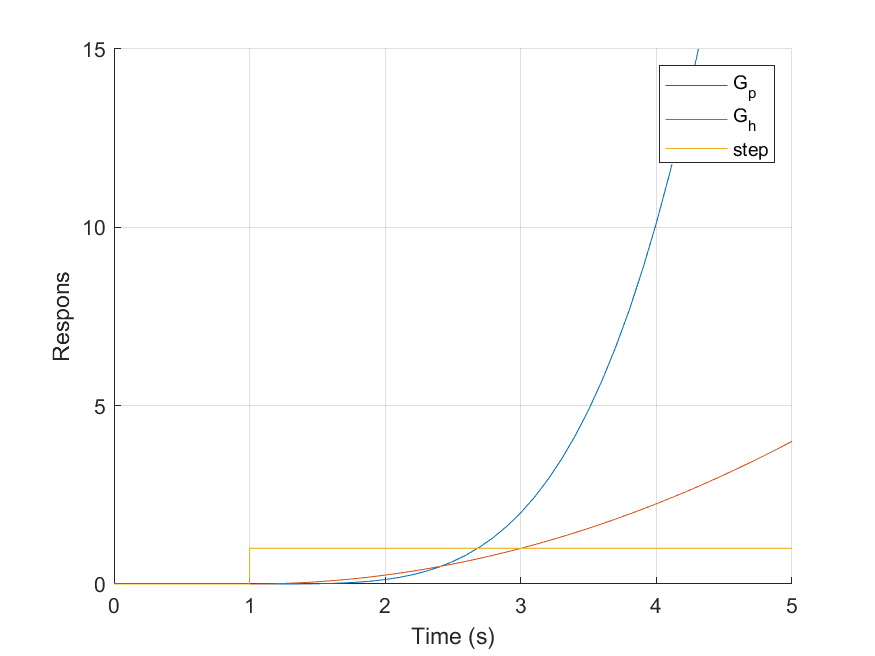
\includegraphics[width=0.8\textwidth]{figures/oppg1_respons.png}
    \caption{Impulsrespons for systemet}
    \label{fig:1}
\end{figure}
\newpage
\subsection{Oppgave 2}
\textbf{(a)}
\begin{figure}
    \centering
    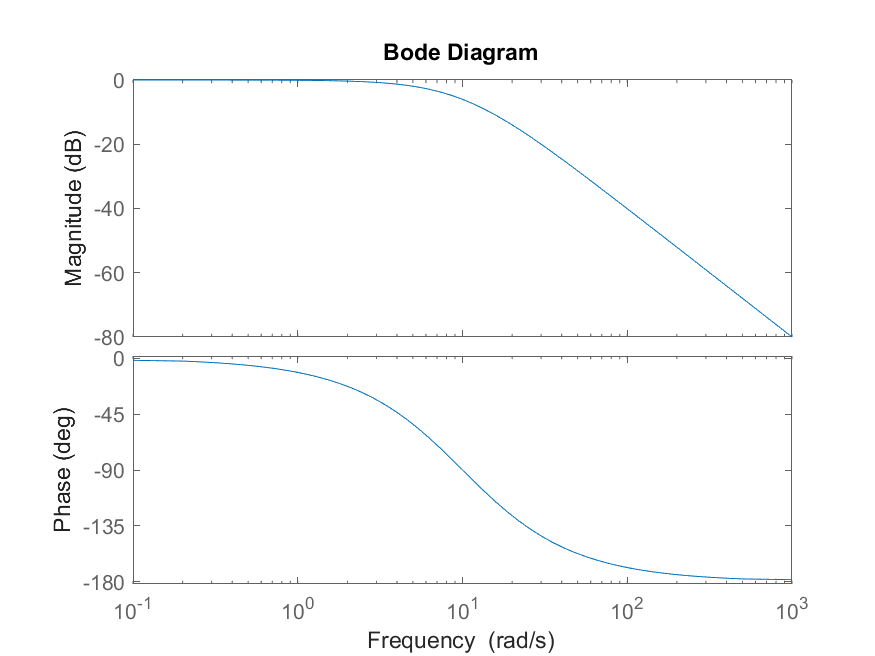
\includegraphics[width=0.8\textwidth]{figures/oppg2_bode.png}
    \caption{Bodeplot for systemet}
    \label{fig:2}
\end{figure}
Grunnet leddet $s^2+\omega_0$ i nevnerer tyder det på at $\hat{u}_\theta$ er en PD-regulator.
Vi forsøker med $\hat{u}_\theta(s) = f\hat{\theta}_{ref} - k_p\hat{\theta}(s) - sk_d\hat{\theta}(s)$.
Gitt $\alpha = J^{-1}l$ satt inn i ligning (\ref{eq:4}) og (\ref{eq:6}) får vi
\begin{equation}
    \begin{aligned}
        s^2\hat{\theta}(s) &= \alpha f \hat{\theta}_{ref} - \alpha k_p\hat{\theta}(s) - s \alpha k_d \hat{\theta}(s) \\
        \hat{\theta}(s)(s^2 + \alpha k_d s + \alpha k_p) &= \alpha f \hat{\theta}_{ref} \\
        \hat{\theta}(s) &= \frac{\alpha f}{s^2 + \alpha k_d s + \alpha k_p} \hat{\theta}_{ref} \\
    \end{aligned}
\end{equation}
Ettersom $(s+\omega_0)^2 = s^2 + 2\omega_0 + \omega_0^2$ for vi disse regulatorverdiene.
\begin{equation}
    \begin{aligned}
        f = \frac{\omega_0^2}{\alpha} = \frac{100}{3}, \quad k_d = \frac{2\omega_0}{\alpha} = \frac{20}{3}, \quad k_p = f = \frac{100}{3} \\
    \end{aligned}
\end{equation}
\textbf{(b)} Her starter vi med samme utgangspunkt som i a, men ligning \ref{eq:4} gir oss nå
\begin{equation}
    \begin{aligned}
        s^2\hat{\theta}(s) &= \frac{1}{Ts+1}(\omega_0^2\hat{\theta}_{ref} - 2\omega_0s\hat{\theta}(s) - \omega_0^2\hat{\theta}(s)) \\
        \hat{\theta}(s)(Ts^3 + s^2 + 2s\omega_0 + \omega_0^2) &= \omega_0^2\hat{\theta}_{ref} \\
        \hat{\theta}(s)(Ts^3 + (s+\omega_0)^2) &= \omega_0^2\hat{\theta}_{ref} \\
        \hat{\theta}(s) &= \frac{\omega_0^2}{Ts^3 + (s+\omega_0)^2} \hat{\theta}_{ref} \\
    \end{aligned}
    \label{eq:14}
\end{equation}
\textbf{(c)} Det relevant elementet vi må ta hensyn til er at $0 \le a_2a_1-a_0a_3 $. Dette gir oss
\begin{equation}
    \begin{aligned}
        2\omega_0 - \omega_0^2T  &\ge 0\\
        T &\le \frac{2}{\omega_0} \\
    \end{aligned}
    \label{eq:15}
\end{equation}
Ligning (\ref{eq:15}) viser at $T \in [0, \frac{1}{5})$ for at systemet skal være stabilt. 
Vi plotter derfor system responsen for økende verdier av T. Resultatet er i figur \ref{fig:3}.
Hvor vi ser at for $T < 0.2$ er systemet stabilt og går mot referansen, $T = 0.2$ oscillerer systemet og for $T > 0.2$ 
blir systemet ustabilt. Her kan det også bemerkes at vi får en overshot ved $T=0.1$, noe vi ikke ser ved $T=0$.
\begin{figure}
    \centering
    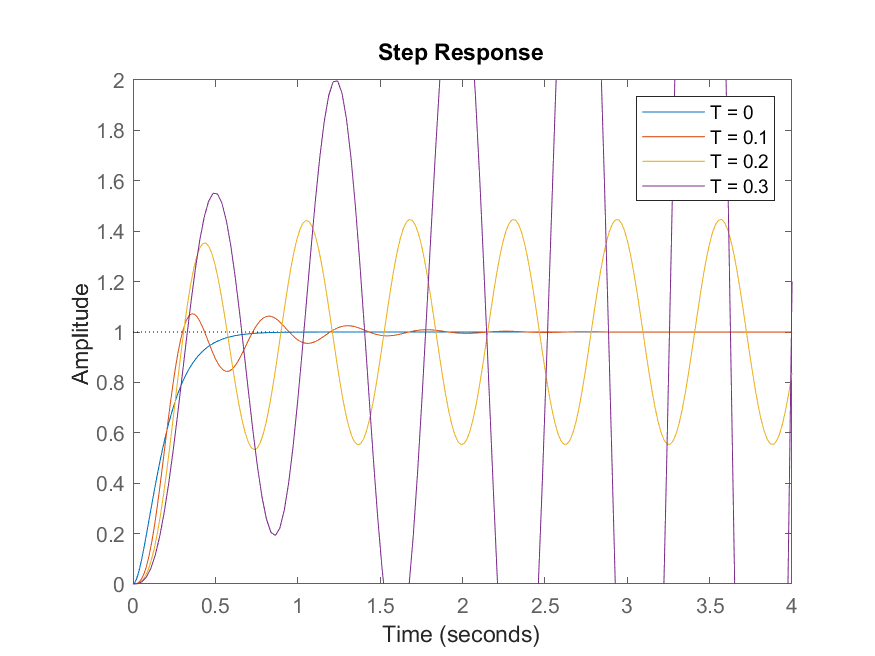
\includegraphics[width=0.8\textwidth]{figures/oppg2_respons.png}
    \label{fig:3}
\end{figure}
\newline
\textbf{(d)} Det er veldig usannsynlig at alle fenomener er tatt med i en matematisk modell.
Dette er fordi det er ekstremt mange små fenomener i et system, som ofte er vanskelig å modellere eller unødvendig å modellere.
\newpage
\subsection{Oppgave 3}
\begin{figure}[H]
    \centering
    \title{\textbf{Dronens bane}}
    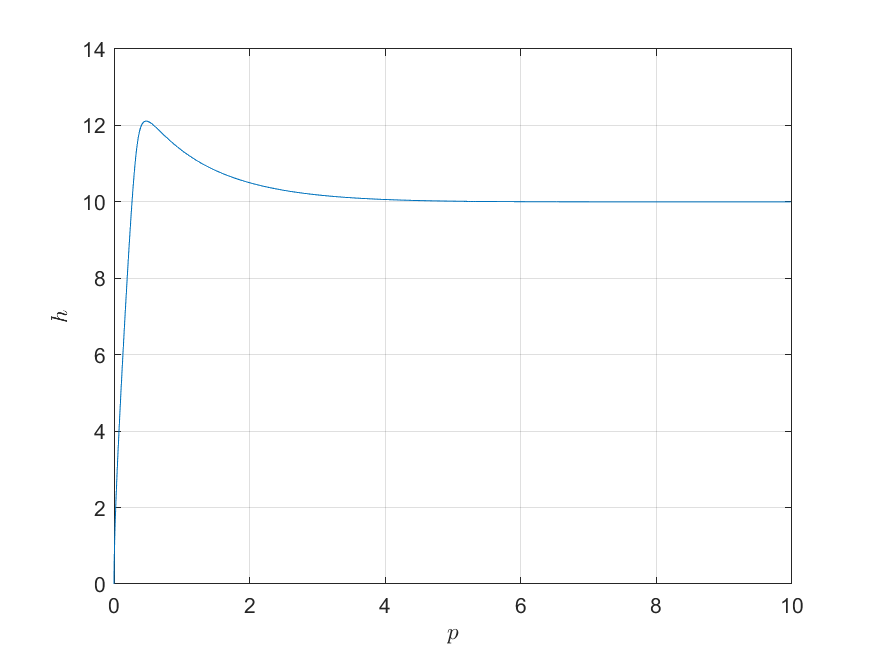
\includegraphics[width=0.8\textwidth]{figures/oppg3_bane.png}
    \caption{Banen dronen følger gitt referansen $(p_{ref}, h_{ref}) = (10, 10)$}
    \label{fig:4}
\end{figure}
\textbf{(a)} Fra sløyfen får vi $\theta_{ref} = K_p(s)(p_{ref} - p)$ og sammen med ligningen $\ddot{p} = g\theta_{ref}$ får vi følgende regulatorutrykk for p.
\begin{equation}
    \begin{aligned}
        \ddot{p} &= g\theta_{ref} \\
        s^2\hat{p}(s) &= g\hat{\theta}_{ref}(s) \\
        s^2\hat{p}(s) &= gK_p(s)(p_{ref} - \hat{p})\\
    \end{aligned}
\end{equation}
Hvor $K_p(s)$ er en PD regulator. Vi ønsker poler i $\lambda_1 = \lambda_2 = -1/4$ som gir en nevner på formen
$s^2 + \frac{1}{2}s + \frac{1}{16}$. Dette gir oss følgende regulatorverdier.
\begin{equation}
    \begin{aligned}
        \hat{p}(s)(s^2 + gk_ds + gk_p) &= K_p(s)p_{ref} \\
        \hat{p}(s) &= \frac{K(s)_pp_{ref}}{s^2 + gk_ds + gk_p} \\
        k_{pd} = \frac{1}{2g}, &\quad k_{pp} = \frac{1}{16g} \\
    \end{aligned}
\end{equation}
\textbf{(b)} Regulatoren har formen $K_h(s) = k_{hp} + k_{hd}s + k_{hi}/s$. Med samme fremgangsmåte som tidligere for vi følgende system
\begin{equation}
    \hat{h} = \frac{K_h(s)h_{ref} + \omega_0}{s^3 + s^2M^{-1}k_{hd} + sM^{-1}k_{hp}+M^{-1}k_{hi}}
\end{equation}
Med poler i $\lambda_1 = 1, \lambda_2 = 2, \lambda_3 = 3$, må vi ha en nevner på formen $s^3 + 6s^2 + 11s + 6$.
Som gir følgende regulatorverdier.
\begin{equation}
    \begin{aligned}
        k_{hp} = 2\cdot11, &\quad k_{hd} = 2\cdot6, &\quad k_{hi} = 2\cdot6 \\
    \end{aligned}
\end{equation}
\textbf{(c)} Regulatorene ble implementert i simulink og resultatene er vist i figur \ref{fig:4}, \ref{fig:5} og \ref{fig:6}. Som viser hhv. dronens bane, høyde og pitch gitt en statisk referanse på
$(p_{ref},h_{ref}) = (10, 10)$.

\begin{figure}
    \centering
    \title{\textbf{Dronens Høyde}}
    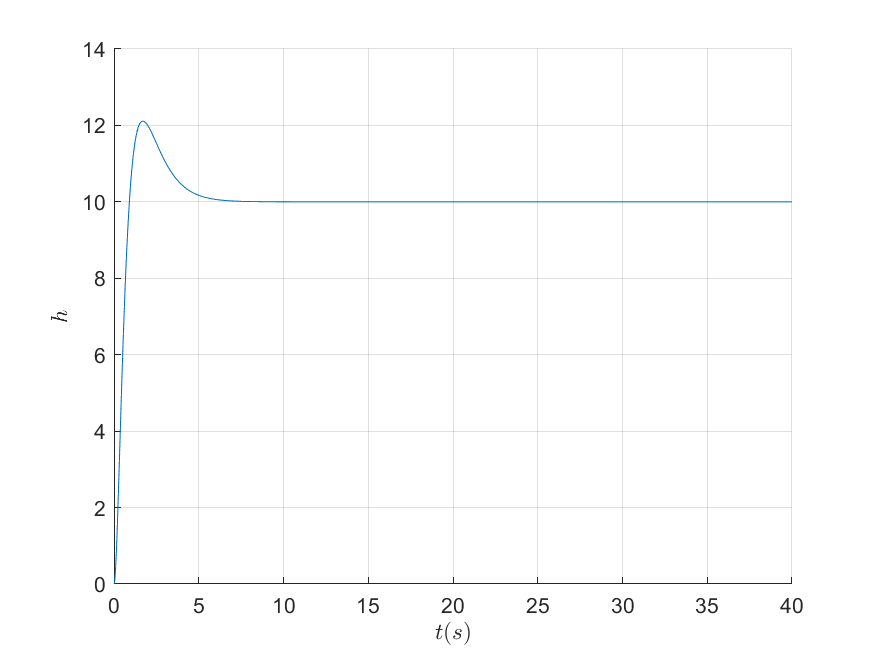
\includegraphics[width=0.8\textwidth]{figures/oppg3_hoyde.png}
    \caption{Høyderespons med gitt regulator}
    \label{fig:5}
\end{figure}
\begin{figure}
    \centering
    \title{\textbf{Dronens Pitch}}
    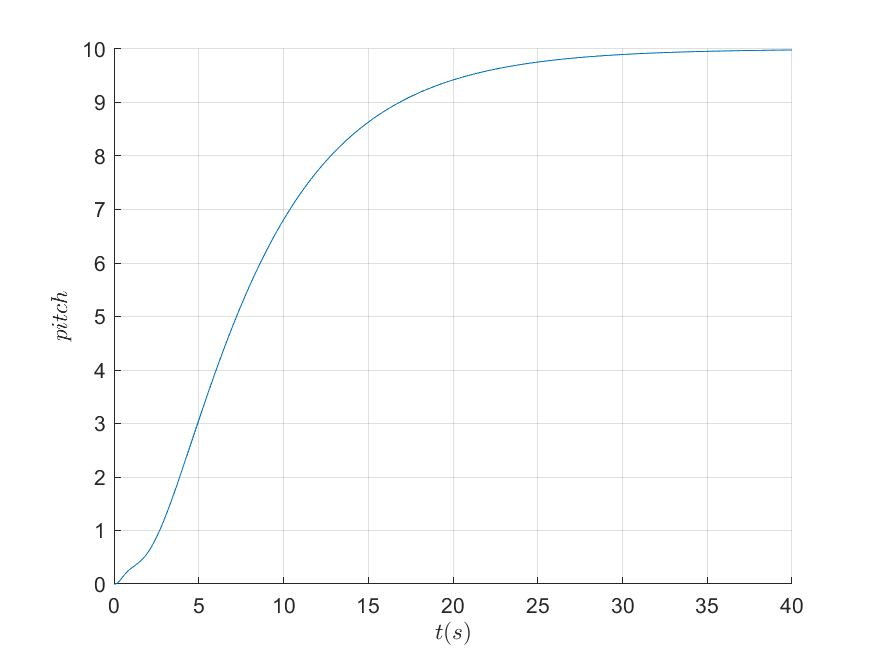
\includegraphics[width=0.8\textwidth]{figures/oppg3_pitch.png}
    \caption{Pitch respons med gitt regulator}
    \label{fig:6}
\end{figure}
\subsection{Oppgave 4}
\textbf{(a)} 
\begin{equation}
    \begin{aligned}
    x_1 = \theta, &\quad x_2 = \dot{\theta} \\
    \dot{x}_1 = \dot{\theta} = x_2, &\quad \dot{x}_2 = \ddot{\theta} = J^{-1}lu_{\theta} \\
    \begin{bmatrix}
        \dot{x}_1 \\
        \dot{x}_2 \\
    \end{bmatrix} = 
    \begin{bmatrix}
        0 & 1 \\
        0 & 0 \\
    \end{bmatrix}&
    \begin{bmatrix}
        x_1 \\
        x_2 \\
    \end{bmatrix} + 
    \begin{bmatrix}
        0 \\
        J^{-1}l \\
    \end{bmatrix}u_{\theta} \\
    \mathbf{\dot{x}} = &\mathbf{Ax} + \mathbf{B}u_{\theta} \\
    \end{aligned}
\end{equation}
\textbf{(b)}
Målematrisene for systemet med bruk av akselerometer og gyroskop er hhv. $ C = \begin{bmatrix} 1 & 0 \end{bmatrix}$ og $C = \begin{bmatrix} 0 & 1 \end{bmatrix}$.
Som gir følgende observerbarhetsmatriser.
\begin{equation}
    \begin{aligned}
        \mathcal{O}_{akselerometer} = \begin{bmatrix} C \\ CA \end{bmatrix} = \begin{bmatrix} 1 & 0 \\ 0 & 1 \end{bmatrix} \\
        \mathcal{O}_{gyroskop} = \begin{bmatrix} C \\ CA \end{bmatrix} = \begin{bmatrix} 0 & 1 \\ 0 & 0 \end{bmatrix} \\
    \end{aligned}
\end{equation}
Her ser vi at kun akselereometeret gir full rang i observerbarhetsmatrisen.
\newline
\textbf{(c)}
For å tune observerforsterkningen kan vi se på feilen til systemet, definert som $\mathbf{e} = \mathbf{x}-\mathbf{\hat{x}}$. Den finner vi ved å gjøre følgende
\begin{equation}
    \begin{aligned}
        \mathbf{\dot{x}} &= \mathbf{Ax} + \mathbf{B}u_{\theta} \\
        \mathbf{\dot{\hat{x}}} &= \mathbf{A}\hat{\mathbf{x}} + \mathbf{B}u_{\theta} + \mathbf{l}(y - \mathbf{C}\hat{\mathbf{x}}) \\
        \mathbf{\dot{e}} &= \mathbf{\dot{x}} - \mathbf{\dot{\hat{x}}} = \mathbf{A}(\mathbf{x} - \hat{\mathbf{x}}) - \mathbf{lC}(\mathbf{x} - \hat{\mathbf{x}}) \\
        \mathbf{\dot{e}} &= (\mathbf{A} - \mathbf{lC})\mathbf{e} \\
        \mathbf{\dot{e}} &=
        \begin{bmatrix}
            -l_1 & 1 \\
            -l_2 & 0 \\
        \end{bmatrix}\mathbf{e} \\
    \end{aligned}
\end{equation}
Den karakteristiske ligninger for systemet er gitt ved $\lambda^2 + l_1\lambda + l_2 = 0$. Dette gir oss l som funksjon av polene til systemet.
\begin{equation}
    \begin{aligned}
        l_1 = -(\lambda_1+\lambda_2), &\quad l_2 = \lambda_1\lambda_2 \\
    \end{aligned}
\end{equation}
\textbf{(d)} Figur \ref{fig:7} og \ref{fig:8} viser estimatorverdiene sammenlignet med de faktiske verdiene med ulike poler.
Valg av l vektes mellom hvor raskt systemet skal konvergere og hvor mye støy som skal ignoreres. Vi ser fra figurene at høye verdier for l bevarer mye støy i estimatoren.
\begin{figure}
    \centering
    \title{\textbf{Estimator mot faktisk verdi}}
    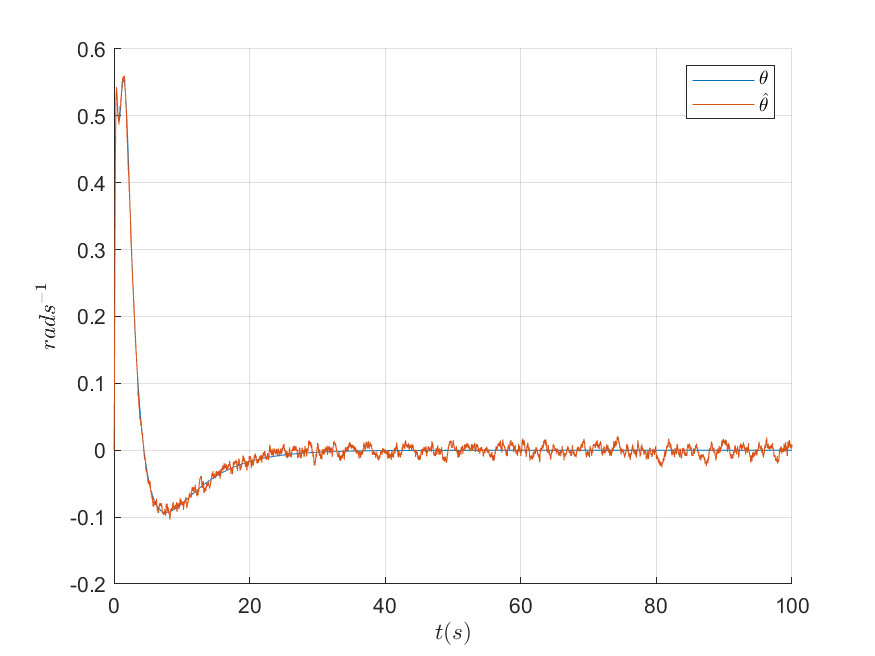
\includegraphics[width=0.8\textwidth]{figures/oppg4_estimator.png}
    \caption{Med $\lambda_1 = \lambda_2 = -2$.}
    \label{fig:7}
\end{figure}
\begin{figure}
    \centering
    \title{\textbf{Estimator mot faktisk verdi}}
    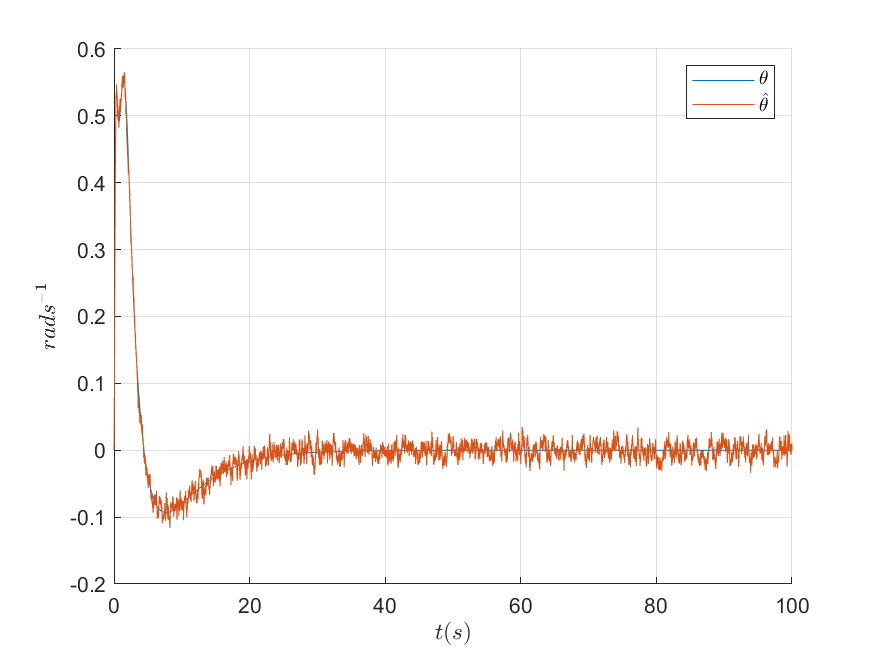
\includegraphics[width=0.8\textwidth]{figures/oppg4_estimator2.png}
    \caption{Med $\lambda_1 = \lambda_2 = -5$.}
    \label{fig:8}
\end{figure}
\newline
\textbf{(e)} Figur \ref{fig:9} viser at dronen fremdeles klarer å følge en gitt referanse selv med estimatorverdier ført inn i regulatoren.
Her er referansene satt til $(p_{ref}, h_{ref}) = (100, 10)$.
\begin{figure}
    \centering
    \title{\textbf{Estimatorverdier i regulator}}
    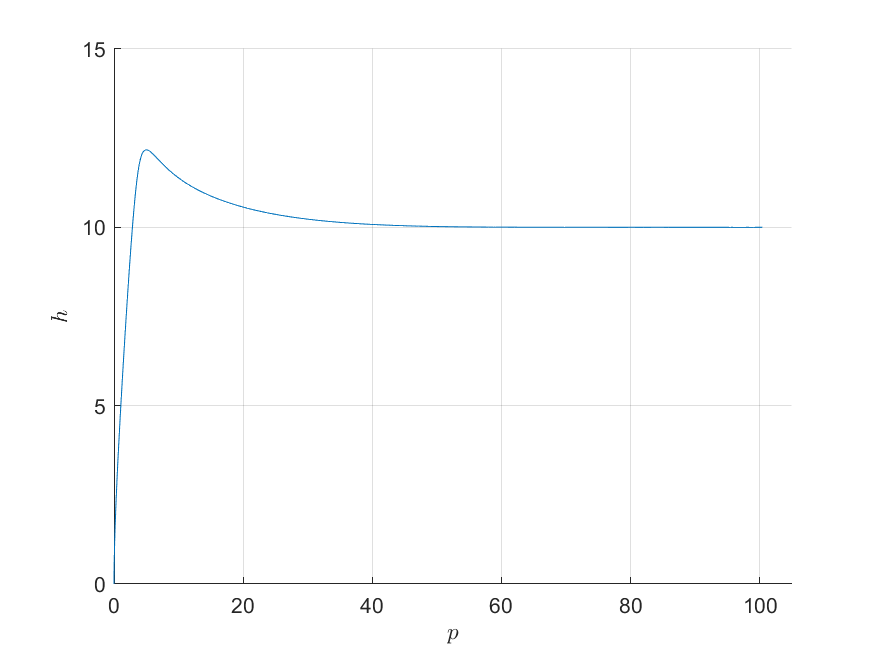
\includegraphics[width=0.8\textwidth]{figures/oppg4_estimator_reg.png}
    \caption{Med $\lambda_1 = -2, \lambda_2 = -5$.}
    \label{fig:9}
\end{figure}
%\printbibliography
\end{document}
